\documentclass[tikz,border=1pt]{standalone}
\usepackage{xcolor}
\usepackage{tikz}
\usetikzlibrary{arrows.meta}
\begin{document}
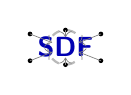
\begin{tikzpicture}
  \draw[thick, gray!55, dashed] (0,0) circle (2.2mm);
  \node[font=\bfseries\sffamily, text=blue!70!black, inner sep=0] at (0,0) {SDF};
  \fill[black] (-4.5mm,1.7mm) circle (0.3mm);
  \draw[->, gray, line width=0.25pt] (-4.5mm,1.7mm) -- (-1.7mm,0.6mm);
  \fill[black] (4.5mm,1.7mm) circle (0.3mm);
  \draw[->, gray, line width=0.25pt] (4.5mm,1.7mm) -- (1.7mm,0.6mm);
  \fill[black] (-4.5mm,-1.7mm) circle (0.3mm);
  \draw[->, gray, line width=0.25pt] (-4.5mm,-1.7mm) -- (-1.7mm,-0.6mm);
  \fill[black] (4.5mm,-1.7mm) circle (0.3mm);
  \draw[->, gray, line width=0.25pt] (4.5mm,-1.7mm) -- (1.7mm,-0.6mm);
  \fill[black] (0,2.2mm) circle (0.3mm);
  \draw[->, gray, line width=0.25pt] (0,2.2mm) -- (0,1.3mm);
  \fill[black] (0,-2.2mm) circle (0.3mm);
  \draw[->, gray, line width=0.25pt] (0,-2.2mm) -- (0,-1.3mm);
\end{tikzpicture}
\end{document}
